
\begin{figure}[ht]
\centering
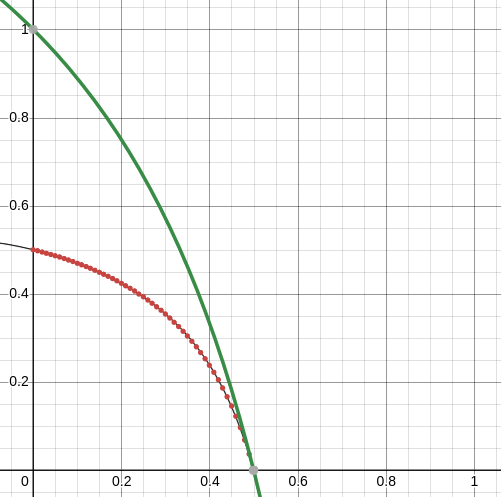
\includegraphics[width=0.55\textwidth]{figures/IMG_ch3/dtctA.png}
\caption{The continuous-time constant $\Ac(p)=(1-2p)/(1-p)$ (green) against
high-precision numerical values of the discrete-time constant $A(p)$ (red points).
Both vanish at $p=\tfrac12$; at $p=0$ the continuous curve starts at $1$ and the
discrete one at $\tfrac12$.}
\label{a:fig:dtct}
\end{figure}

\section{Why the discrete and continuous constants differ}
\label{a:sec:compare}

The question raised by \cref{a:fig:dtct} can now be settled. The two constants are
\begin{equation*}
\Ac(p) = \frac{1-2p}{1-p}\quad\text{(continuous time)},
\qquad
A(p) = \lim_{n\to\infty}\frac{S_n}{(2p)^n}\quad\text{(discrete time)},
\end{equation*}
and the observation was that the first starts at $1$ where the second starts at
$\tfrac12$, yet halving the first does not superpose the curves.

\Cref{a:prop:bounds} explains this completely. What holds is not
$A=\tfrac12\Ac$ but the strict inequality $A>\tfrac12\Ac$, and the inequality is
attained only in the limit $p\to0$. Combining \cref{a:eq:Aasym,a:eq:Acts}, the ratio
runs monotonically across the interval:
\begin{equation}
\label{a:eq:ratiolimits}
\frac{A(p)}{\Ac(p)} \;\longrightarrow\; \tfrac12 \quad(p\to0),
\qquad
\frac{A(p)}{\Ac(p)} \;\longrightarrow\; 1 \quad(p\to\tfrac12^-),
\end{equation}
taking the values $0.503$, $0.528$, $0.619$, $0.798$, $0.928$ and $0.988$ at
$p=0.01,\,0.1,\,0.3,\,0.45,\,0.49,\,0.499$. No constant factor will do, because the
ratio is not constant.

The two endpoints have clean interpretations, and they are different in kind.

At $p\to0$ the factor of two is a counting effect. In the binary discrete model an
individual leaves either nothing or two offspring, so a surviving population is
always even (\cref{a:prop:parity}); deep in the subcritical regime, conditioning on
survival means conditioning on a population of exactly two, and the
quasi-stationary mean is $2$. In the continuous-time model a survivor is a single
individual that has not yet died, so the quasi-stationary mean is $1$. The
reciprocals are $\tfrac12$ and $1$, and there is the discrepancy.

At $p\to\tfrac12^-$ the factor disappears, because both constants are governed by
the same critical scaling. Expanding \cref{a:eq:Acts} near $p=\tfrac12$ gives
$\Ac(p) = (1-2p)/(1-p)\to2(1-2p)$, which is precisely \cref{a:eq:Aasym}. Near
criticality the discreteness of the generational clock stops mattering; what
survives is the universal $2\varepsilon$ behaviour, and the two models agree to
leading order.

The discrete curve is therefore squeezed between $\tfrac12\Ac$ and its own critical
asymptote, hugging the former at one end and the latter at the other. That is the
whole content of \cref{a:fig:dtct}.

